% Created by tikzDevice version 0.8.1 on 2015-05-29 17:33:18
% !TEX encoding = UTF-8 Unicode
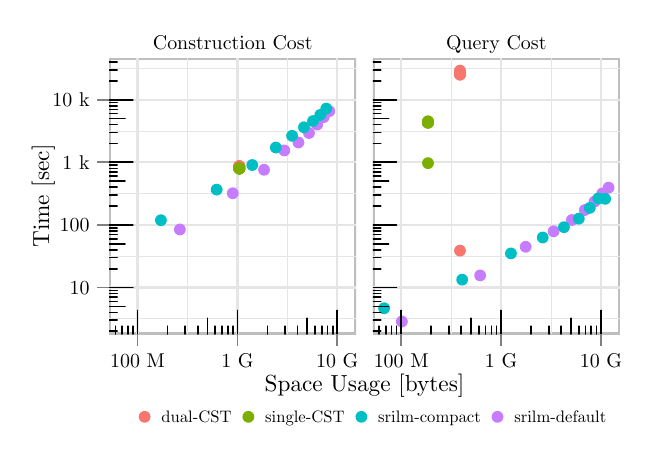
\begin{tikzpicture}[x=1pt,y=1pt]
\definecolor{fillColor}{RGB}{255,255,255}
\path[use as bounding box,fill=fillColor,fill opacity=0.00] (0,0) rectangle (216.81,144.54);
\begin{scope}
\path[clip] (  0.00,  0.00) rectangle (216.81,144.54);
\definecolor{fillColor}{RGB}{255,255,255}

\path[fill=fillColor] (  0.00,  0.00) rectangle (216.81,144.54);
\end{scope}
\begin{scope}
\path[clip] ( 29.47,133.56) rectangle (118.71,144.54);

\path[] ( 29.47,133.56) rectangle (118.71,144.54);
\definecolor{drawColor}{RGB}{0,0,0}

\node[text=drawColor,anchor=base,inner sep=0pt, outer sep=0pt, scale=  0.72] at ( 74.09,136.57) {Construction Cost};
\end{scope}
\begin{scope}
\path[clip] (124.73,133.56) rectangle (213.96,144.54);

\path[] (124.73,133.56) rectangle (213.96,144.54);
\definecolor{drawColor}{RGB}{0,0,0}

\node[text=drawColor,anchor=base,inner sep=0pt, outer sep=0pt, scale=  0.72] at (169.35,136.57) {Query Cost};
\end{scope}
\begin{scope}
\path[clip] ( 29.47, 33.84) rectangle (118.71,133.56);
\definecolor{drawColor}{RGB}{190,190,190}

\path[draw=drawColor,line width= 1.5pt,line join=round,line cap=round] ( 29.47, 33.84) rectangle (118.71,133.56);
\definecolor{drawColor}{gray}{0.90}

\path[draw=drawColor,line width= 0.3pt,line join=round] ( 29.47, 39.32) --
	(118.71, 39.32);

\path[draw=drawColor,line width= 0.3pt,line join=round] ( 29.47, 61.95) --
	(118.71, 61.95);

\path[draw=drawColor,line width= 0.3pt,line join=round] ( 29.47, 84.57) --
	(118.71, 84.57);

\path[draw=drawColor,line width= 0.3pt,line join=round] ( 29.47,107.20) --
	(118.71,107.20);

\path[draw=drawColor,line width= 0.3pt,line join=round] ( 29.47,129.83) --
	(118.71,129.83);

\path[draw=drawColor,line width= 0.3pt,line join=round] ( 57.75, 33.84) --
	( 57.75,133.56);

\path[draw=drawColor,line width= 0.3pt,line join=round] ( 93.84, 33.84) --
	( 93.84,133.56);

\path[draw=drawColor,line width= 0.8pt,line join=round] ( 29.47, 50.64) --
	(118.71, 50.64);

\path[draw=drawColor,line width= 0.8pt,line join=round] ( 29.47, 73.26) --
	(118.71, 73.26);

\path[draw=drawColor,line width= 0.8pt,line join=round] ( 29.47, 95.89) --
	(118.71, 95.89);

\path[draw=drawColor,line width= 0.8pt,line join=round] ( 29.47,118.51) --
	(118.71,118.51);

\path[draw=drawColor,line width= 0.8pt,line join=round] ( 39.70, 33.84) --
	( 39.70,133.56);

\path[draw=drawColor,line width= 0.8pt,line join=round] ( 75.79, 33.84) --
	( 75.79,133.56);

\path[draw=drawColor,line width= 0.8pt,line join=round] (111.88, 33.84) --
	(111.88,133.56);
\definecolor{fillColor}{RGB}{199,124,255}

\path[fill=fillColor] ( 54.99, 71.63) circle (  2.13);

\path[fill=fillColor] ( 74.11, 84.71) circle (  2.13);

\path[fill=fillColor] ( 85.41, 93.19) circle (  2.13);

\path[fill=fillColor] ( 92.74,100.17) circle (  2.13);

\path[fill=fillColor] ( 97.84,103.05) circle (  2.13);

\path[fill=fillColor] (101.64,106.47) circle (  2.13);

\path[fill=fillColor] (104.61,109.52) circle (  2.13);

\path[fill=fillColor] (107.01,112.23) circle (  2.13);

\path[fill=fillColor] (109.00,114.39) circle (  2.13);
\definecolor{fillColor}{RGB}{0,191,196}

\path[fill=fillColor] ( 48.15, 74.96) circle (  2.13);

\path[fill=fillColor] ( 68.30, 86.02) circle (  2.13);

\path[fill=fillColor] ( 81.15, 94.91) circle (  2.13);

\path[fill=fillColor] ( 89.67,101.23) circle (  2.13);

\path[fill=fillColor] ( 95.54,105.46) circle (  2.13);

\path[fill=fillColor] ( 99.83,108.54) circle (  2.13);

\path[fill=fillColor] (103.11,110.80) circle (  2.13);

\path[fill=fillColor] (105.73,113.01) circle (  2.13);

\path[fill=fillColor] (107.88,115.29) circle (  2.13);
\definecolor{fillColor}{RGB}{248,118,109}

\path[fill=fillColor] ( 76.48, 94.42) circle (  2.13);

\path[fill=fillColor] ( 76.48, 94.42) circle (  2.13);

\path[fill=fillColor] ( 76.48, 94.42) circle (  2.13);

\path[fill=fillColor] ( 76.48, 94.42) circle (  2.13);

\path[fill=fillColor] ( 76.48, 94.42) circle (  2.13);

\path[fill=fillColor] ( 76.48, 94.42) circle (  2.13);

\path[fill=fillColor] ( 76.48, 94.42) circle (  2.13);

\path[fill=fillColor] ( 76.48, 94.42) circle (  2.13);

\path[fill=fillColor] ( 76.48, 94.42) circle (  2.13);
\definecolor{fillColor}{RGB}{124,174,0}

\path[fill=fillColor] ( 76.48, 93.66) circle (  2.13);

\path[fill=fillColor] ( 76.48, 93.66) circle (  2.13);

\path[fill=fillColor] ( 76.48, 93.66) circle (  2.13);

\path[fill=fillColor] ( 76.48, 93.66) circle (  2.13);

\path[fill=fillColor] ( 76.48, 93.66) circle (  2.13);

\path[fill=fillColor] ( 76.48, 93.66) circle (  2.13);

\path[fill=fillColor] ( 76.48, 93.66) circle (  2.13);

\path[fill=fillColor] ( 76.48, 93.66) circle (  2.13);

\path[fill=fillColor] ( 76.48, 93.66) circle (  2.13);
\definecolor{drawColor}{RGB}{0,0,0}

\path[draw=drawColor,line width= 0.6pt,line join=round,line cap=round] (  3.61, 33.84) -- (  3.61, 42.37);

\path[draw=drawColor,line width= 0.6pt,line join=round,line cap=round] ( 14.48, 33.84) -- ( 14.48, 36.68);

\path[draw=drawColor,line width= 0.6pt,line join=round,line cap=round] ( 20.83, 33.84) -- ( 20.83, 36.68);

\path[draw=drawColor,line width= 0.6pt,line join=round,line cap=round] ( 25.34, 33.84) -- ( 25.34, 36.68);

\path[draw=drawColor,line width= 0.6pt,line join=round,line cap=round] ( 28.84, 33.84) -- ( 28.84, 39.53);

\path[draw=drawColor,line width= 0.6pt,line join=round,line cap=round] ( 31.70, 33.84) -- ( 31.70, 36.68);

\path[draw=drawColor,line width= 0.6pt,line join=round,line cap=round] ( 34.11, 33.84) -- ( 34.11, 36.68);

\path[draw=drawColor,line width= 0.6pt,line join=round,line cap=round] ( 36.21, 33.84) -- ( 36.21, 36.68);

\path[draw=drawColor,line width= 0.6pt,line join=round,line cap=round] ( 38.05, 33.84) -- ( 38.05, 36.68);

\path[draw=drawColor,line width= 0.6pt,line join=round,line cap=round] ( 39.70, 33.84) -- ( 39.70, 42.37);

\path[draw=drawColor,line width= 0.6pt,line join=round,line cap=round] ( 50.57, 33.84) -- ( 50.57, 36.68);

\path[draw=drawColor,line width= 0.6pt,line join=round,line cap=round] ( 56.92, 33.84) -- ( 56.92, 36.68);

\path[draw=drawColor,line width= 0.6pt,line join=round,line cap=round] ( 61.43, 33.84) -- ( 61.43, 36.68);

\path[draw=drawColor,line width= 0.6pt,line join=round,line cap=round] ( 64.93, 33.84) -- ( 64.93, 39.53);

\path[draw=drawColor,line width= 0.6pt,line join=round,line cap=round] ( 67.79, 33.84) -- ( 67.79, 36.68);

\path[draw=drawColor,line width= 0.6pt,line join=round,line cap=round] ( 70.20, 33.84) -- ( 70.20, 36.68);

\path[draw=drawColor,line width= 0.6pt,line join=round,line cap=round] ( 72.30, 33.84) -- ( 72.30, 36.68);

\path[draw=drawColor,line width= 0.6pt,line join=round,line cap=round] ( 74.14, 33.84) -- ( 74.14, 36.68);

\path[draw=drawColor,line width= 0.6pt,line join=round,line cap=round] ( 75.79, 33.84) -- ( 75.79, 42.37);

\path[draw=drawColor,line width= 0.6pt,line join=round,line cap=round] ( 86.66, 33.84) -- ( 86.66, 36.68);

\path[draw=drawColor,line width= 0.6pt,line join=round,line cap=round] ( 93.01, 33.84) -- ( 93.01, 36.68);

\path[draw=drawColor,line width= 0.6pt,line join=round,line cap=round] ( 97.52, 33.84) -- ( 97.52, 36.68);

\path[draw=drawColor,line width= 0.6pt,line join=round,line cap=round] (101.02, 33.84) -- (101.02, 39.53);

\path[draw=drawColor,line width= 0.6pt,line join=round,line cap=round] (103.88, 33.84) -- (103.88, 36.68);

\path[draw=drawColor,line width= 0.6pt,line join=round,line cap=round] (106.29, 33.84) -- (106.29, 36.68);

\path[draw=drawColor,line width= 0.6pt,line join=round,line cap=round] (108.39, 33.84) -- (108.39, 36.68);

\path[draw=drawColor,line width= 0.6pt,line join=round,line cap=round] (110.23, 33.84) -- (110.23, 36.68);

\path[draw=drawColor,line width= 0.6pt,line join=round,line cap=round] (111.88, 33.84) -- (111.88, 42.37);

\path[draw=drawColor,line width= 0.6pt,line join=round,line cap=round] (122.75, 33.84) -- (122.75, 36.68);

\path[draw=drawColor,line width= 0.6pt,line join=round,line cap=round] (129.10, 33.84) -- (129.10, 36.68);

\path[draw=drawColor,line width= 0.6pt,line join=round,line cap=round] (133.61, 33.84) -- (133.61, 36.68);

\path[draw=drawColor,line width= 0.6pt,line join=round,line cap=round] (137.11, 33.84) -- (137.11, 39.53);

\path[draw=drawColor,line width= 0.6pt,line join=round,line cap=round] (139.97, 33.84) -- (139.97, 36.68);

\path[draw=drawColor,line width= 0.6pt,line join=round,line cap=round] (142.38, 33.84) -- (142.38, 36.68);

\path[draw=drawColor,line width= 0.6pt,line join=round,line cap=round] (144.48, 33.84) -- (144.48, 36.68);

\path[draw=drawColor,line width= 0.6pt,line join=round,line cap=round] (146.32, 33.84) -- (146.32, 36.68);

\path[draw=drawColor,line width= 0.6pt,line join=round,line cap=round] (147.98, 33.84) -- (147.98, 42.37);

\path[draw=drawColor,line width= 0.6pt,line join=round,line cap=round] ( 29.47, 28.01) -- ( 38.01, 28.01);

\path[draw=drawColor,line width= 0.6pt,line join=round,line cap=round] ( 29.47, 34.82) -- ( 32.32, 34.82);

\path[draw=drawColor,line width= 0.6pt,line join=round,line cap=round] ( 29.47, 38.81) -- ( 32.32, 38.81);

\path[draw=drawColor,line width= 0.6pt,line join=round,line cap=round] ( 29.47, 41.63) -- ( 32.32, 41.63);

\path[draw=drawColor,line width= 0.6pt,line join=round,line cap=round] ( 29.47, 43.83) -- ( 35.16, 43.83);

\path[draw=drawColor,line width= 0.6pt,line join=round,line cap=round] ( 29.47, 45.62) -- ( 32.32, 45.62);

\path[draw=drawColor,line width= 0.6pt,line join=round,line cap=round] ( 29.47, 47.13) -- ( 32.32, 47.13);

\path[draw=drawColor,line width= 0.6pt,line join=round,line cap=round] ( 29.47, 48.44) -- ( 32.32, 48.44);

\path[draw=drawColor,line width= 0.6pt,line join=round,line cap=round] ( 29.47, 49.60) -- ( 32.32, 49.60);

\path[draw=drawColor,line width= 0.6pt,line join=round,line cap=round] ( 29.47, 50.64) -- ( 38.01, 50.64);

\path[draw=drawColor,line width= 0.6pt,line join=round,line cap=round] ( 29.47, 57.45) -- ( 32.32, 57.45);

\path[draw=drawColor,line width= 0.6pt,line join=round,line cap=round] ( 29.47, 61.43) -- ( 32.32, 61.43);

\path[draw=drawColor,line width= 0.6pt,line join=round,line cap=round] ( 29.47, 64.26) -- ( 32.32, 64.26);

\path[draw=drawColor,line width= 0.6pt,line join=round,line cap=round] ( 29.47, 66.45) -- ( 35.16, 66.45);

\path[draw=drawColor,line width= 0.6pt,line join=round,line cap=round] ( 29.47, 68.24) -- ( 32.32, 68.24);

\path[draw=drawColor,line width= 0.6pt,line join=round,line cap=round] ( 29.47, 69.76) -- ( 32.32, 69.76);

\path[draw=drawColor,line width= 0.6pt,line join=round,line cap=round] ( 29.47, 71.07) -- ( 32.32, 71.07);

\path[draw=drawColor,line width= 0.6pt,line join=round,line cap=round] ( 29.47, 72.23) -- ( 32.32, 72.23);

\path[draw=drawColor,line width= 0.6pt,line join=round,line cap=round] ( 29.47, 73.26) -- ( 38.01, 73.26);

\path[draw=drawColor,line width= 0.6pt,line join=round,line cap=round] ( 29.47, 80.07) -- ( 32.32, 80.07);

\path[draw=drawColor,line width= 0.6pt,line join=round,line cap=round] ( 29.47, 84.06) -- ( 32.32, 84.06);

\path[draw=drawColor,line width= 0.6pt,line join=round,line cap=round] ( 29.47, 86.88) -- ( 32.32, 86.88);

\path[draw=drawColor,line width= 0.6pt,line join=round,line cap=round] ( 29.47, 89.08) -- ( 35.16, 89.08);

\path[draw=drawColor,line width= 0.6pt,line join=round,line cap=round] ( 29.47, 90.87) -- ( 32.32, 90.87);

\path[draw=drawColor,line width= 0.6pt,line join=round,line cap=round] ( 29.47, 92.38) -- ( 32.32, 92.38);

\path[draw=drawColor,line width= 0.6pt,line join=round,line cap=round] ( 29.47, 93.69) -- ( 32.32, 93.69);

\path[draw=drawColor,line width= 0.6pt,line join=round,line cap=round] ( 29.47, 94.85) -- ( 32.32, 94.85);

\path[draw=drawColor,line width= 0.6pt,line join=round,line cap=round] ( 29.47, 95.89) -- ( 38.01, 95.89);

\path[draw=drawColor,line width= 0.6pt,line join=round,line cap=round] ( 29.47,102.70) -- ( 32.32,102.70);

\path[draw=drawColor,line width= 0.6pt,line join=round,line cap=round] ( 29.47,106.68) -- ( 32.32,106.68);

\path[draw=drawColor,line width= 0.6pt,line join=round,line cap=round] ( 29.47,109.51) -- ( 32.32,109.51);

\path[draw=drawColor,line width= 0.6pt,line join=round,line cap=round] ( 29.47,111.70) -- ( 35.16,111.70);

\path[draw=drawColor,line width= 0.6pt,line join=round,line cap=round] ( 29.47,113.49) -- ( 32.32,113.49);

\path[draw=drawColor,line width= 0.6pt,line join=round,line cap=round] ( 29.47,115.01) -- ( 32.32,115.01);

\path[draw=drawColor,line width= 0.6pt,line join=round,line cap=round] ( 29.47,116.32) -- ( 32.32,116.32);

\path[draw=drawColor,line width= 0.6pt,line join=round,line cap=round] ( 29.47,117.48) -- ( 32.32,117.48);

\path[draw=drawColor,line width= 0.6pt,line join=round,line cap=round] ( 29.47,118.51) -- ( 38.01,118.51);

\path[draw=drawColor,line width= 0.6pt,line join=round,line cap=round] ( 29.47,125.32) -- ( 32.32,125.32);

\path[draw=drawColor,line width= 0.6pt,line join=round,line cap=round] ( 29.47,129.31) -- ( 32.32,129.31);

\path[draw=drawColor,line width= 0.6pt,line join=round,line cap=round] ( 29.47,132.13) -- ( 32.32,132.13);

\path[draw=drawColor,line width= 0.6pt,line join=round,line cap=round] ( 29.47,134.33) -- ( 35.16,134.33);

\path[draw=drawColor,line width= 0.6pt,line join=round,line cap=round] ( 29.47,136.12) -- ( 32.32,136.12);

\path[draw=drawColor,line width= 0.6pt,line join=round,line cap=round] ( 29.47,137.63) -- ( 32.32,137.63);

\path[draw=drawColor,line width= 0.6pt,line join=round,line cap=round] ( 29.47,138.95) -- ( 32.32,138.95);

\path[draw=drawColor,line width= 0.6pt,line join=round,line cap=round] ( 29.47,140.10) -- ( 32.32,140.10);

\path[draw=drawColor,line width= 0.6pt,line join=round,line cap=round] ( 29.47,141.14) -- ( 38.01,141.14);
\end{scope}
\begin{scope}
\path[clip] (124.73, 33.84) rectangle (213.96,133.56);
\definecolor{drawColor}{RGB}{190,190,190}

\path[draw=drawColor,line width= 1.5pt,line join=round,line cap=round] (124.73, 33.84) rectangle (213.96,133.56);
\definecolor{drawColor}{gray}{0.90}

\path[draw=drawColor,line width= 0.3pt,line join=round] (124.73, 39.32) --
	(213.96, 39.32);

\path[draw=drawColor,line width= 0.3pt,line join=round] (124.73, 61.95) --
	(213.96, 61.95);

\path[draw=drawColor,line width= 0.3pt,line join=round] (124.73, 84.57) --
	(213.96, 84.57);

\path[draw=drawColor,line width= 0.3pt,line join=round] (124.73,107.20) --
	(213.96,107.20);

\path[draw=drawColor,line width= 0.3pt,line join=round] (124.73,129.83) --
	(213.96,129.83);

\path[draw=drawColor,line width= 0.3pt,line join=round] (153.01, 33.84) --
	(153.01,133.56);

\path[draw=drawColor,line width= 0.3pt,line join=round] (189.10, 33.84) --
	(189.10,133.56);

\path[draw=drawColor,line width= 0.8pt,line join=round] (124.73, 50.64) --
	(213.96, 50.64);

\path[draw=drawColor,line width= 0.8pt,line join=round] (124.73, 73.26) --
	(213.96, 73.26);

\path[draw=drawColor,line width= 0.8pt,line join=round] (124.73, 95.89) --
	(213.96, 95.89);

\path[draw=drawColor,line width= 0.8pt,line join=round] (124.73,118.51) --
	(213.96,118.51);

\path[draw=drawColor,line width= 0.8pt,line join=round] (134.96, 33.84) --
	(134.96,133.56);

\path[draw=drawColor,line width= 0.8pt,line join=round] (171.05, 33.84) --
	(171.05,133.56);

\path[draw=drawColor,line width= 0.8pt,line join=round] (207.14, 33.84) --
	(207.14,133.56);
\definecolor{fillColor}{RGB}{199,124,255}

\path[fill=fillColor] (135.22, 38.37) circle (  2.13);

\path[fill=fillColor] (163.50, 55.01) circle (  2.13);

\path[fill=fillColor] (179.96, 65.36) circle (  2.13);

\path[fill=fillColor] (190.04, 70.95) circle (  2.13);

\path[fill=fillColor] (196.64, 75.04) circle (  2.13);

\path[fill=fillColor] (201.32, 78.65) circle (  2.13);

\path[fill=fillColor] (204.85, 81.72) circle (  2.13);

\path[fill=fillColor] (207.64, 84.65) circle (  2.13);

\path[fill=fillColor] (209.91, 86.74) circle (  2.13);
\definecolor{fillColor}{RGB}{0,191,196}

\path[fill=fillColor] (128.79, 43.15) circle (  2.13);

\path[fill=fillColor] (157.00, 53.48) circle (  2.13);

\path[fill=fillColor] (174.63, 62.97) circle (  2.13);

\path[fill=fillColor] (186.12, 68.71) circle (  2.13);

\path[fill=fillColor] (193.78, 72.45) circle (  2.13);

\path[fill=fillColor] (199.15, 75.52) circle (  2.13);

\path[fill=fillColor] (203.12, 79.40) circle (  2.13);

\path[fill=fillColor] (206.20, 82.82) circle (  2.13);

\path[fill=fillColor] (208.67, 82.68) circle (  2.13);
\definecolor{fillColor}{RGB}{248,118,109}

\path[fill=fillColor] (156.21, 63.97) circle (  2.13);

\path[fill=fillColor] (156.21,127.87) circle (  2.13);

\path[fill=fillColor] (156.21,128.09) circle (  2.13);

\path[fill=fillColor] (156.21,128.71) circle (  2.13);

\path[fill=fillColor] (156.21,128.60) circle (  2.13);

\path[fill=fillColor] (156.21,129.03) circle (  2.13);

\path[fill=fillColor] (156.21,127.61) circle (  2.13);

\path[fill=fillColor] (156.21,127.61) circle (  2.13);

\path[fill=fillColor] (156.21,127.61) circle (  2.13);
\definecolor{fillColor}{RGB}{124,174,0}

\path[fill=fillColor] (144.65, 95.59) circle (  2.13);

\path[fill=fillColor] (144.65,110.17) circle (  2.13);

\path[fill=fillColor] (144.65,110.41) circle (  2.13);

\path[fill=fillColor] (144.65,110.39) circle (  2.13);

\path[fill=fillColor] (144.65,110.29) circle (  2.13);

\path[fill=fillColor] (144.65,110.34) circle (  2.13);

\path[fill=fillColor] (144.65,110.73) circle (  2.13);

\path[fill=fillColor] (144.65,110.21) circle (  2.13);

\path[fill=fillColor] (144.65,110.40) circle (  2.13);
\definecolor{drawColor}{RGB}{0,0,0}

\path[draw=drawColor,line width= 0.6pt,line join=round,line cap=round] ( 98.87, 33.84) -- ( 98.87, 42.37);

\path[draw=drawColor,line width= 0.6pt,line join=round,line cap=round] (109.74, 33.84) -- (109.74, 36.68);

\path[draw=drawColor,line width= 0.6pt,line join=round,line cap=round] (116.09, 33.84) -- (116.09, 36.68);

\path[draw=drawColor,line width= 0.6pt,line join=round,line cap=round] (120.60, 33.84) -- (120.60, 36.68);

\path[draw=drawColor,line width= 0.6pt,line join=round,line cap=round] (124.10, 33.84) -- (124.10, 39.53);

\path[draw=drawColor,line width= 0.6pt,line join=round,line cap=round] (126.96, 33.84) -- (126.96, 36.68);

\path[draw=drawColor,line width= 0.6pt,line join=round,line cap=round] (129.37, 33.84) -- (129.37, 36.68);

\path[draw=drawColor,line width= 0.6pt,line join=round,line cap=round] (131.46, 33.84) -- (131.46, 36.68);

\path[draw=drawColor,line width= 0.6pt,line join=round,line cap=round] (133.31, 33.84) -- (133.31, 36.68);

\path[draw=drawColor,line width= 0.6pt,line join=round,line cap=round] (134.96, 33.84) -- (134.96, 42.37);

\path[draw=drawColor,line width= 0.6pt,line join=round,line cap=round] (145.83, 33.84) -- (145.83, 36.68);

\path[draw=drawColor,line width= 0.6pt,line join=round,line cap=round] (152.18, 33.84) -- (152.18, 36.68);

\path[draw=drawColor,line width= 0.6pt,line join=round,line cap=round] (156.69, 33.84) -- (156.69, 36.68);

\path[draw=drawColor,line width= 0.6pt,line join=round,line cap=round] (160.19, 33.84) -- (160.19, 39.53);

\path[draw=drawColor,line width= 0.6pt,line join=round,line cap=round] (163.05, 33.84) -- (163.05, 36.68);

\path[draw=drawColor,line width= 0.6pt,line join=round,line cap=round] (165.46, 33.84) -- (165.46, 36.68);

\path[draw=drawColor,line width= 0.6pt,line join=round,line cap=round] (167.55, 33.84) -- (167.55, 36.68);

\path[draw=drawColor,line width= 0.6pt,line join=round,line cap=round] (169.40, 33.84) -- (169.40, 36.68);

\path[draw=drawColor,line width= 0.6pt,line join=round,line cap=round] (171.05, 33.84) -- (171.05, 42.37);

\path[draw=drawColor,line width= 0.6pt,line join=round,line cap=round] (181.92, 33.84) -- (181.92, 36.68);

\path[draw=drawColor,line width= 0.6pt,line join=round,line cap=round] (188.27, 33.84) -- (188.27, 36.68);

\path[draw=drawColor,line width= 0.6pt,line join=round,line cap=round] (192.78, 33.84) -- (192.78, 36.68);

\path[draw=drawColor,line width= 0.6pt,line join=round,line cap=round] (196.28, 33.84) -- (196.28, 39.53);

\path[draw=drawColor,line width= 0.6pt,line join=round,line cap=round] (199.14, 33.84) -- (199.14, 36.68);

\path[draw=drawColor,line width= 0.6pt,line join=round,line cap=round] (201.55, 33.84) -- (201.55, 36.68);

\path[draw=drawColor,line width= 0.6pt,line join=round,line cap=round] (203.64, 33.84) -- (203.64, 36.68);

\path[draw=drawColor,line width= 0.6pt,line join=round,line cap=round] (205.49, 33.84) -- (205.49, 36.68);

\path[draw=drawColor,line width= 0.6pt,line join=round,line cap=round] (207.14, 33.84) -- (207.14, 42.37);

\path[draw=drawColor,line width= 0.6pt,line join=round,line cap=round] (124.73, 28.01) -- (133.27, 28.01);

\path[draw=drawColor,line width= 0.6pt,line join=round,line cap=round] (124.73, 34.82) -- (127.58, 34.82);

\path[draw=drawColor,line width= 0.6pt,line join=round,line cap=round] (124.73, 38.81) -- (127.58, 38.81);

\path[draw=drawColor,line width= 0.6pt,line join=round,line cap=round] (124.73, 41.63) -- (127.58, 41.63);

\path[draw=drawColor,line width= 0.6pt,line join=round,line cap=round] (124.73, 43.83) -- (130.42, 43.83);

\path[draw=drawColor,line width= 0.6pt,line join=round,line cap=round] (124.73, 45.62) -- (127.58, 45.62);

\path[draw=drawColor,line width= 0.6pt,line join=round,line cap=round] (124.73, 47.13) -- (127.58, 47.13);

\path[draw=drawColor,line width= 0.6pt,line join=round,line cap=round] (124.73, 48.44) -- (127.58, 48.44);

\path[draw=drawColor,line width= 0.6pt,line join=round,line cap=round] (124.73, 49.60) -- (127.58, 49.60);

\path[draw=drawColor,line width= 0.6pt,line join=round,line cap=round] (124.73, 50.64) -- (133.27, 50.64);

\path[draw=drawColor,line width= 0.6pt,line join=round,line cap=round] (124.73, 57.45) -- (127.58, 57.45);

\path[draw=drawColor,line width= 0.6pt,line join=round,line cap=round] (124.73, 61.43) -- (127.58, 61.43);

\path[draw=drawColor,line width= 0.6pt,line join=round,line cap=round] (124.73, 64.26) -- (127.58, 64.26);

\path[draw=drawColor,line width= 0.6pt,line join=round,line cap=round] (124.73, 66.45) -- (130.42, 66.45);

\path[draw=drawColor,line width= 0.6pt,line join=round,line cap=round] (124.73, 68.24) -- (127.58, 68.24);

\path[draw=drawColor,line width= 0.6pt,line join=round,line cap=round] (124.73, 69.76) -- (127.58, 69.76);

\path[draw=drawColor,line width= 0.6pt,line join=round,line cap=round] (124.73, 71.07) -- (127.58, 71.07);

\path[draw=drawColor,line width= 0.6pt,line join=round,line cap=round] (124.73, 72.23) -- (127.58, 72.23);

\path[draw=drawColor,line width= 0.6pt,line join=round,line cap=round] (124.73, 73.26) -- (133.27, 73.26);

\path[draw=drawColor,line width= 0.6pt,line join=round,line cap=round] (124.73, 80.07) -- (127.58, 80.07);

\path[draw=drawColor,line width= 0.6pt,line join=round,line cap=round] (124.73, 84.06) -- (127.58, 84.06);

\path[draw=drawColor,line width= 0.6pt,line join=round,line cap=round] (124.73, 86.88) -- (127.58, 86.88);

\path[draw=drawColor,line width= 0.6pt,line join=round,line cap=round] (124.73, 89.08) -- (130.42, 89.08);

\path[draw=drawColor,line width= 0.6pt,line join=round,line cap=round] (124.73, 90.87) -- (127.58, 90.87);

\path[draw=drawColor,line width= 0.6pt,line join=round,line cap=round] (124.73, 92.38) -- (127.58, 92.38);

\path[draw=drawColor,line width= 0.6pt,line join=round,line cap=round] (124.73, 93.69) -- (127.58, 93.69);

\path[draw=drawColor,line width= 0.6pt,line join=round,line cap=round] (124.73, 94.85) -- (127.58, 94.85);

\path[draw=drawColor,line width= 0.6pt,line join=round,line cap=round] (124.73, 95.89) -- (133.27, 95.89);

\path[draw=drawColor,line width= 0.6pt,line join=round,line cap=round] (124.73,102.70) -- (127.58,102.70);

\path[draw=drawColor,line width= 0.6pt,line join=round,line cap=round] (124.73,106.68) -- (127.58,106.68);

\path[draw=drawColor,line width= 0.6pt,line join=round,line cap=round] (124.73,109.51) -- (127.58,109.51);

\path[draw=drawColor,line width= 0.6pt,line join=round,line cap=round] (124.73,111.70) -- (130.42,111.70);

\path[draw=drawColor,line width= 0.6pt,line join=round,line cap=round] (124.73,113.49) -- (127.58,113.49);

\path[draw=drawColor,line width= 0.6pt,line join=round,line cap=round] (124.73,115.01) -- (127.58,115.01);

\path[draw=drawColor,line width= 0.6pt,line join=round,line cap=round] (124.73,116.32) -- (127.58,116.32);

\path[draw=drawColor,line width= 0.6pt,line join=round,line cap=round] (124.73,117.48) -- (127.58,117.48);

\path[draw=drawColor,line width= 0.6pt,line join=round,line cap=round] (124.73,118.51) -- (133.27,118.51);

\path[draw=drawColor,line width= 0.6pt,line join=round,line cap=round] (124.73,125.32) -- (127.58,125.32);

\path[draw=drawColor,line width= 0.6pt,line join=round,line cap=round] (124.73,129.31) -- (127.58,129.31);

\path[draw=drawColor,line width= 0.6pt,line join=round,line cap=round] (124.73,132.13) -- (127.58,132.13);

\path[draw=drawColor,line width= 0.6pt,line join=round,line cap=round] (124.73,134.33) -- (130.42,134.33);

\path[draw=drawColor,line width= 0.6pt,line join=round,line cap=round] (124.73,136.12) -- (127.58,136.12);

\path[draw=drawColor,line width= 0.6pt,line join=round,line cap=round] (124.73,137.63) -- (127.58,137.63);

\path[draw=drawColor,line width= 0.6pt,line join=round,line cap=round] (124.73,138.95) -- (127.58,138.95);

\path[draw=drawColor,line width= 0.6pt,line join=round,line cap=round] (124.73,140.10) -- (127.58,140.10);

\path[draw=drawColor,line width= 0.6pt,line join=round,line cap=round] (124.73,141.14) -- (133.27,141.14);
\end{scope}
\begin{scope}
\path[clip] (  0.00,  0.00) rectangle (216.81,144.54);
\definecolor{drawColor}{RGB}{0,0,0}

\node[text=drawColor,anchor=base east,inner sep=0pt, outer sep=0pt, scale=  0.72] at ( 22.36, 48.16) {10};

\node[text=drawColor,anchor=base east,inner sep=0pt, outer sep=0pt, scale=  0.72] at ( 22.36, 70.78) {100};

\node[text=drawColor,anchor=base east,inner sep=0pt, outer sep=0pt, scale=  0.72] at ( 22.36, 93.41) {1 k};

\node[text=drawColor,anchor=base east,inner sep=0pt, outer sep=0pt, scale=  0.72] at ( 22.36,116.03) {10 k};
\end{scope}
\begin{scope}
\path[clip] (  0.00,  0.00) rectangle (216.81,144.54);
\definecolor{drawColor}{gray}{0.50}

\path[draw=drawColor,line width= 0.6pt,line join=round] ( 25.20, 50.64) --
	( 29.47, 50.64);

\path[draw=drawColor,line width= 0.6pt,line join=round] ( 25.20, 73.26) --
	( 29.47, 73.26);

\path[draw=drawColor,line width= 0.6pt,line join=round] ( 25.20, 95.89) --
	( 29.47, 95.89);

\path[draw=drawColor,line width= 0.6pt,line join=round] ( 25.20,118.51) --
	( 29.47,118.51);
\end{scope}
\begin{scope}
\path[clip] (  0.00,  0.00) rectangle (216.81,144.54);
\definecolor{drawColor}{gray}{0.50}

\path[draw=drawColor,line width= 0.6pt,line join=round] ( 39.70, 29.57) --
	( 39.70, 33.84);

\path[draw=drawColor,line width= 0.6pt,line join=round] ( 75.79, 29.57) --
	( 75.79, 33.84);

\path[draw=drawColor,line width= 0.6pt,line join=round] (111.88, 29.57) --
	(111.88, 33.84);
\end{scope}
\begin{scope}
\path[clip] (  0.00,  0.00) rectangle (216.81,144.54);
\definecolor{drawColor}{RGB}{0,0,0}

\node[text=drawColor,anchor=base,inner sep=0pt, outer sep=0pt, scale=  0.72] at ( 39.70, 21.77) {100 M};

\node[text=drawColor,anchor=base,inner sep=0pt, outer sep=0pt, scale=  0.72] at ( 75.79, 21.77) {1 G};

\node[text=drawColor,anchor=base,inner sep=0pt, outer sep=0pt, scale=  0.72] at (111.88, 21.77) {10 G};
\end{scope}
\begin{scope}
\path[clip] (  0.00,  0.00) rectangle (216.81,144.54);
\definecolor{drawColor}{gray}{0.50}

\path[draw=drawColor,line width= 0.6pt,line join=round] (134.96, 29.57) --
	(134.96, 33.84);

\path[draw=drawColor,line width= 0.6pt,line join=round] (171.05, 29.57) --
	(171.05, 33.84);

\path[draw=drawColor,line width= 0.6pt,line join=round] (207.14, 29.57) --
	(207.14, 33.84);
\end{scope}
\begin{scope}
\path[clip] (  0.00,  0.00) rectangle (216.81,144.54);
\definecolor{drawColor}{RGB}{0,0,0}

\node[text=drawColor,anchor=base,inner sep=0pt, outer sep=0pt, scale=  0.72] at (134.96, 21.77) {100 M};

\node[text=drawColor,anchor=base,inner sep=0pt, outer sep=0pt, scale=  0.72] at (171.05, 21.77) {1 G};

\node[text=drawColor,anchor=base,inner sep=0pt, outer sep=0pt, scale=  0.72] at (207.14, 21.77) {10 G};
\end{scope}
\begin{scope}
\path[clip] (  0.00,  0.00) rectangle (216.81,144.54);
\definecolor{drawColor}{RGB}{0,0,0}

\node[text=drawColor,anchor=base,inner sep=0pt, outer sep=0pt, scale=  0.84] at (121.72, 12.97) {Space Usage [bytes]};
\end{scope}
\begin{scope}
\path[clip] (  0.00,  0.00) rectangle (216.81,144.54);
\definecolor{drawColor}{RGB}{0,0,0}

\node[text=drawColor,rotate= 90.00,anchor=base,inner sep=0pt, outer sep=0pt, scale=  0.84] at (  7.76, 83.70) {Time [sec]};
\end{scope}
\begin{scope}
\path[clip] (  0.00,  0.00) rectangle (216.81,144.54);
\definecolor{fillColor}{RGB}{248,118,109}

\path[fill=fillColor] ( 42.26,  3.92) circle (  2.13);
\end{scope}
\begin{scope}
\path[clip] (  0.00,  0.00) rectangle (216.81,144.54);
\definecolor{fillColor}{RGB}{124,174,0}

\path[fill=fillColor] ( 79.74,  3.92) circle (  2.13);
\end{scope}
\begin{scope}
\path[clip] (  0.00,  0.00) rectangle (216.81,144.54);
\definecolor{fillColor}{RGB}{0,191,196}

\path[fill=fillColor] (120.58,  3.92) circle (  2.13);
\end{scope}
\begin{scope}
\path[clip] (  0.00,  0.00) rectangle (216.81,144.54);
\definecolor{fillColor}{RGB}{199,124,255}

\path[fill=fillColor] (169.77,  3.92) circle (  2.13);
\end{scope}
\begin{scope}
\path[clip] (  0.00,  0.00) rectangle (216.81,144.54);
\definecolor{drawColor}{RGB}{0,0,0}

\node[text=drawColor,anchor=base west,inner sep=0pt, outer sep=0pt, scale=  0.60] at ( 48.34,  1.86) {dual-CST};
\end{scope}
\begin{scope}
\path[clip] (  0.00,  0.00) rectangle (216.81,144.54);
\definecolor{drawColor}{RGB}{0,0,0}

\node[text=drawColor,anchor=base west,inner sep=0pt, outer sep=0pt, scale=  0.60] at ( 85.81,  1.86) {single-CST};
\end{scope}
\begin{scope}
\path[clip] (  0.00,  0.00) rectangle (216.81,144.54);
\definecolor{drawColor}{RGB}{0,0,0}

\node[text=drawColor,anchor=base west,inner sep=0pt, outer sep=0pt, scale=  0.60] at (126.66,  1.86) {srilm-compact};
\end{scope}
\begin{scope}
\path[clip] (  0.00,  0.00) rectangle (216.81,144.54);
\definecolor{drawColor}{RGB}{0,0,0}

\node[text=drawColor,anchor=base west,inner sep=0pt, outer sep=0pt, scale=  0.60] at (175.85,  1.86) {srilm-default};
\end{scope}
\end{tikzpicture}
